\documentclass[sigconf]{acmart}

\usepackage{hyperref}

%\usepackage{endfloat}
%\renewcommand{\efloatseparator}{\mbox{}} % no new page between figures

\usepackage{booktabs} % For formal tables

\settopmatter{printacmref=false} % Removes citation information below abstract
\renewcommand\footnotetextcopyrightpermission[1]{} % removes footnote with conference information in first column
\pagestyle{plain} % removes running headers


\begin{document}
\title{Big Data Applications and Analysis in Maternal Death During Childbirth in the United States}


\author{Elena Kirzhner}
\affiliation{%
  \institution{Indiana University Bloomington}
  \streetaddress{3209 E 10th St}
  \city{Bloomington} 
  \state{Indiana} 
  \postcode{47408}
}
\email{ekirzhne@iu.edu}


\begin{abstract}

Maternal mortality rate in the United States had increased by more than 25 percent from 2000 to 2014. Reducing maternal death during childbirth requires in-depth examination of isolated causes of death. With the major growth of big data and applications, it is possible to collect, analyze and compare specific maternal death causes and contributing factors to predict who's susceptible to fatality and what can be done to prevent it. It will help to develop focused clinical and public health prevention programs.
\end{abstract}

\keywords{i523, hid320, Big Data Applications and Analytics, Data Science, Maternal Mortality}

\maketitle

\section{Introduction}

Maternity death is rising for unclear reasons in United States. USA is the only developed nation where that rate is increasing and getting worse.
 
American women are more likely to die from childbirth than women in any other high developed country. Based on research and analysis by the Center for Disease Control and Prevention \cite{bacak2006state}, maternal death greatly increased from 2000-2014 and more than half of such incidents could have been prevented with the current medical technology.

Most of the cases were result of medical error and unprepared hospitals. Doctor\textquotesingle s ability to protect the health of mothers in childbirth is a basic measure of a society\textquotesingle s development. Yet every year in the United States 700 to 900 women die from pregnancy or childbirth-related causes, and some 65,000 nearly die. By many measures, the worst record in the developed world \cite{world2012trends} and \cite{amnesty2010deadly}.

We have ability to prevent it, by analyzing each cause and predict with monitoring the cases and usage of the Big Data and Analytics. 

Statistical research for 2010 put America in the 50th place; the lowest of all developed nations for maternal death during childbirth\cite{bingham2011maternal}. Figure \ref{fig:figure1} shows Maternal Mortality ratio by developed countries per 100,000 live births \cite{maron2015has}.

\begin{figure}
  \centering
  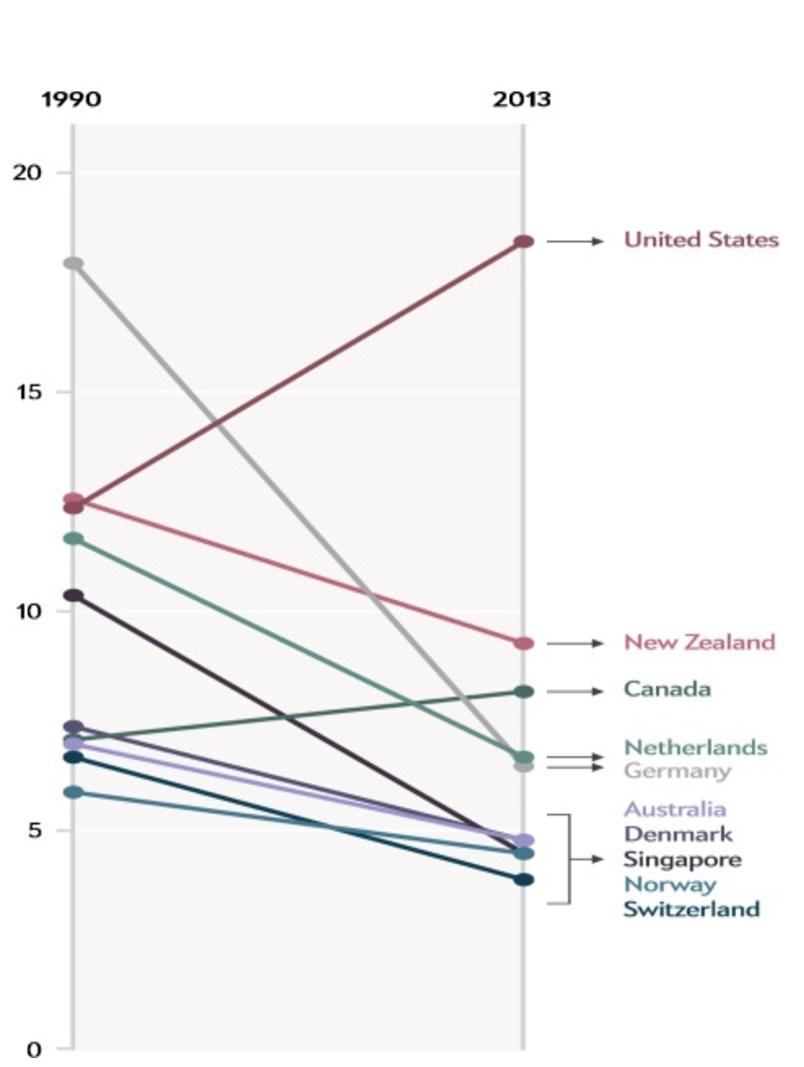
\includegraphics[width=\columnwidth]{images/figure1.pdf}
  \caption{A comparison of maternal mortality ratio in the United States with those of some developed countries between 1990 and 2013 \cite{maron2015has}.} \label{fig:figure1} 
\end{figure}

From 1990 to 2014 pregnancy related death increased by 1.7\% while worldwide that rate decreased by 1.3\%. Thus, proper calculation shows that maternity mortality rate practically doubled in the last decade.

Figure \ref{fig:figure2} shows percent change in maternal deaths per 100,000 live births, from 1990-2013 \cite{kassebaum2016global}.

\begin{figure}
  \centering
  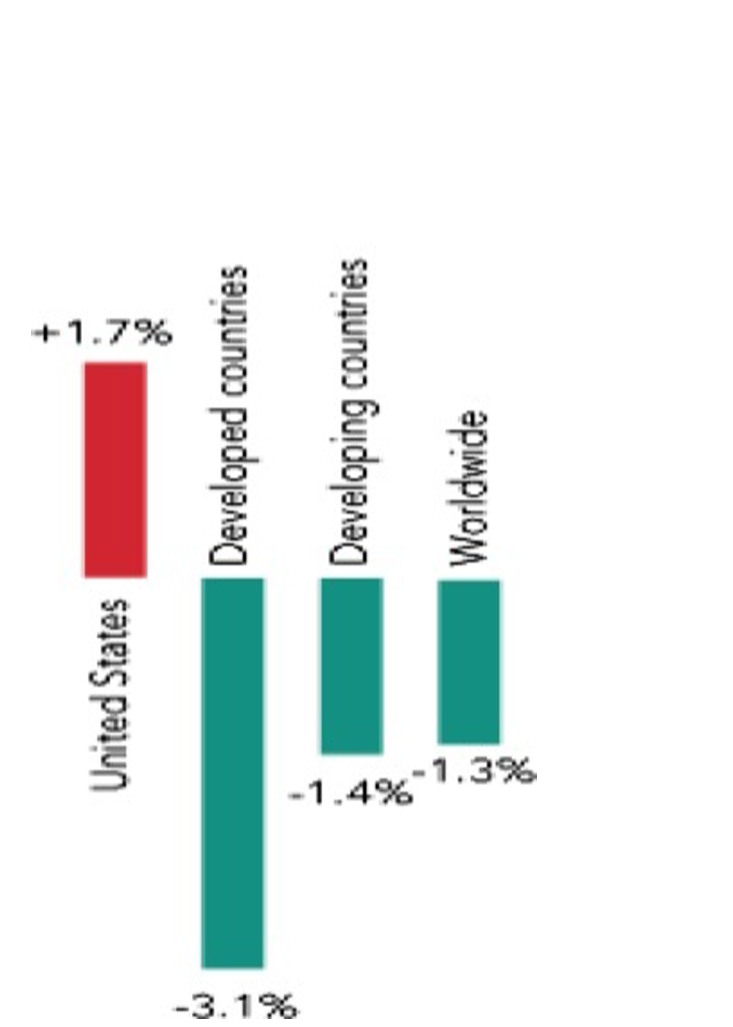
\includegraphics[width=0.5\columnwidth]{images/figure2.pdf}
  \caption{Percentage change in Maternal Mortality Rate between 1990 and 2013 in the United States, worldwide, developed and developing countries \cite{kassebaum2016global}.} \label{fig:figure2} 
\end{figure}

Women giving birth in Asia have lower risk to die than those giving birth in United States \cite{world2012trends}.

Currently, researches are inconclusive, as to why the rate is rising in USA. Multiple variables are being taken into account, such as race, age and economic status \cite{creanga2012race}.

\subsection{Definition}

According to the National Center for Health Statistics, Pregnancy Mortality Surveillance System and the International Classification of Disease, to properly analyze data, causes of death during child birth were categorized and defined \cite{callaghan2012overview} as follows:


1. Pregnancy related death - death during the first 42 days after giving birth that is directly related to pregnancy and health care. Not related to any accidents outside of the pregnancy.
   


2. Maternal fatality ratio - death caused by pregnancy for every 100,000 pregnancy occurrences.


\subsection{Monitoring}

The National Center for Health Statistics requires all states on annual basis to provide death certificates with causes of maternal death. This data is analyzed and compared against international statistics \cite{hoyert2007maternal} and \cite{creanga2014maternal}.

Additionally, Pregnancy Mortality Surveillance System was implemented in 1896, because of limited pregnancy death related records  \cite{horon2011effectiveness}. This system was created to record and analyze all pregnancy related deaths. Every year, this group sends a request to all 50 states to provide death certificate copies for those who died during childbirth and pregnancy. This data is stored and further analyzed by trained doctors, specialists and data scientists. That group coined a new term ''pregnancy-related mortality'' \cite{callaghan2012overview}. This information is being released in Center for Disease Control and Prevention Morbidity and Mortality Weekly reports and their website \cite{neggers2016trends}. Deaths related to pregnancy from 1998-2010 were published in Obstetrics and Gynecology journal \cite{schulz1994assessing}. Furthermore, since launching the program, monitoring and analyzing the data, rate has dramatically increased from 7.2 deaths per 100,000 births in 1987 to 17.8 deaths per 100,000 births in 2011 \cite{neggers2016trends}. Figure \ref{fig:figure3} shows changes in pregnancy related mortality ratio in United States from 1987-2011 \cite{centers2014pregnancyrelated}.

\begin{figure}
  \centering
  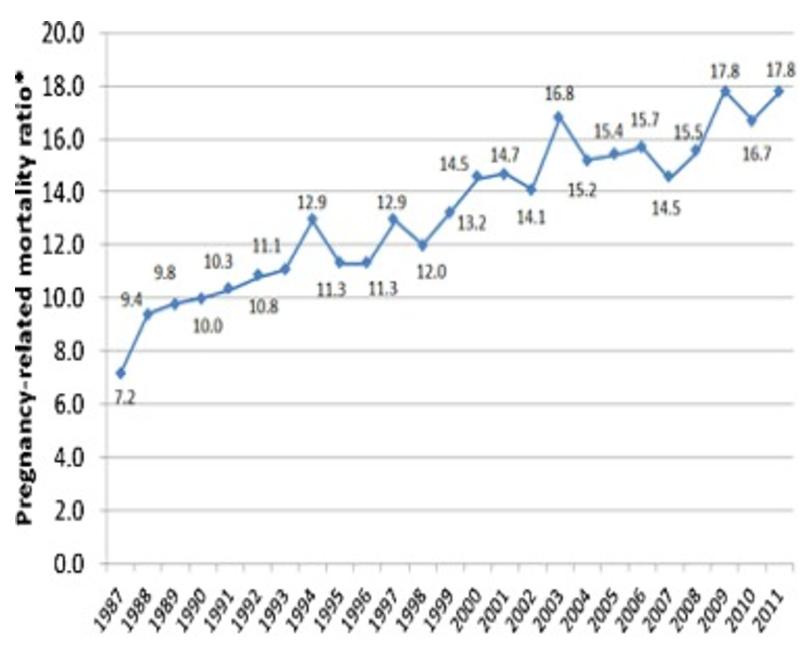
\includegraphics[width=0.5\textwidth]{images/figure3.pdf}
  \caption{Changes in pregnancy related mortality ratio in United States from 1987-2011 \cite{centers2014pregnancyrelated}.} \label{fig:figure3} 
\end{figure}


\section{Big Data Usage And How It Can Help}

The maternity deaths cases are well suited for a big data usage and solution. We have large amount of unstructured data. It could be used on advanced level for further examination. The data could be simplified and accessible to everyone including patients and doctors. However, there are not enough expertise to use it and limited financial resources. On the other hand, some experts say that it is good to have unstructured or raw data, because it was not modified and could add real value to healthcare analytics. It is fresh and ready to be consumed \cite{dineshkumar2016big}.

The causes of maternity death are not yet identified. We have only limited amount of data that was analyzed \cite{creanga2012race}.

Moving forward, we need to understand and organize pregnancy related deaths and causes. Figure out structure and and identify risks by race ethnicity, economic status and age. Professional examination and generated analysis of structured and unstructured data could help with preventing causes of pregnancy related death.

\subsection{Who Is Already Doing It}

Over 200 healthcare applications were developed since 2010. Number of healthcare providers have already benefited from big data by concentrating on the fundamental structure of the big data. 
Few examples below:

 Kaiser Permanente adapted new system called HealthConnect, it communicates new data between collected information about patients and treatments. The implemented system have helped to save more than one billion dollars from lowering patients visits to doctor\textquotesingle s office \cite{groves2016big}.

 Blue Shield of California adapted NantHealth and improved outcomes between patients and hospitals by communicating information about the visits, patient health history and hospitals. It helped to provide most effective and cheaper treatments for chronicle illness with preventive care and communications between doctors and patients \cite{groves2016big}.

 The Lancet Journal done similar study on October 8, 2016 that called ''Global, regional, and national levels of maternal mortality, 1990-2015: a systematic analysis for the Global Burden of Disease Study 2015'' \cite{kassebaum2016global}. They used a standardized process to identify, extract and process all relevant data sources. Uniformed algorithms were applied to identify age category, year category, and location specific patterns of failure and hidden records for vital registration, as well as patterns of deaths misrepresentation \cite{mcginnis2013best}.

\subsection{Internet Of Things}

Big Data and the Internet Of Things is a growing system that allows convergence of physical equipment that transfers data and communicate with other devices and digital networks tearing down silo walls between operational technology  and  information technology. In conjunction with big data it allows for extraction of valuable information.

It could be used to  monitor patient's health and their pregnancy risks  such as diabetes level or blood pressure. It could also track prescribed medicine, it is especially useful for patients without health insurances \cite{kassebaum2016global}. 

\subsection{Predictive Analytics}

Many tools are being utilized for predictive analytics usage, such as data mining, statistics and historical facts. It is being used to analyze given information and generate predictions and outcomes for future and unforeseen events. Stored data could be useful, pregnant women\textquotesingle s  information could be shared between doctors and hospitals to be diagnosed in advance, improving number of healthy pregnancies. By being able to analyze relevant data, pregnancy risks could be predicted and provide women with safer and better pregnancy outcomes. The more analyzed data we have, the sooner it will reduce the mortality rates and we'll be able to diagnose each case. Special emergency kits with appropriate medicine could be supplied to each hospital and doctor's office for individual patient.

Huge amount of data is being generated daily and it comes from different sources in variety of shapes and sizes. Pregnancy related issues are being collected through social media, forums, blood tests, pharmaceutical companies, doctor visits, ultrasounds, hospitals, emails and so on. Our life became very digital. Currently, every doctor\textquotesingle s  visit is being recorded digitally, and electronically health records are being stored at health-care insurance departments and hospital facilities. These records are playing important part of research and scientific analysis.

\subsection{Crunching Big Data}

US government is focusing on research and transforming healthcare knowledge. Big data software becoming accessible and being developed for efficiency and made it easier to collect and analyze data from different sources. One of the best options for the data analysis is to input it into Hadoop system to make a more scaleable analysis with that. As of today, it is one of the most popular data management option. Additionally, it is one of the largest systems that is being used by many companies. Its ability to handle multiple amount of data from different sources, makes it productive and provides possibility to get more accurate causes and reasons of any health issues. Hadoop system is an open source software for distributed storage of large datasets on computer clusters and visualization. There are two main features; Hadoop Distributed File System, which responsible for files storage, and MapReduce, which generates and processes the data. The primary function of this programs is the capability to process huge amount of unstructured data and print out analyzed information. This system is all about handling the Big Data \cite{dittrich2012efficient}.

\section{Conclusion}

Pregnancy-related mortality findings should be studied and cross analyzed with the latest and advanced technology. It will provide a new view and value, resulting clarification and better health management. 

Additionally, it will decrease same errors and doctors faults and prevent maternity death and its causes.

All these years, there was not enough information that was structured for deeper understanding and analysis. It can be improved. Big Data massively grows daily, useful information is everywhere around us; including emails, doctor\textquotesingle s notes, lab tests, health insurances, ultrasounds, social media and pharmaceuticals .

Latest and fastest platforms such as Hadoop, have the ability to transform and improve the healthcare, store data and analyze huge mass of information from separate sources.

Doctors, medical staff and patients could use that information to improve and achieve better outcomes for pregnant mothers and prevent death. 
In addition, it will lower medical costs.


\begin{acks}

  The author would like to thank Dr. Gregor von Laszewski and Miao Jiang for their help, support and suggestions to write this paper.

\end{acks}

\bibliographystyle{ACM-Reference-Format}
\bibliography{report} 

\end{document}
